
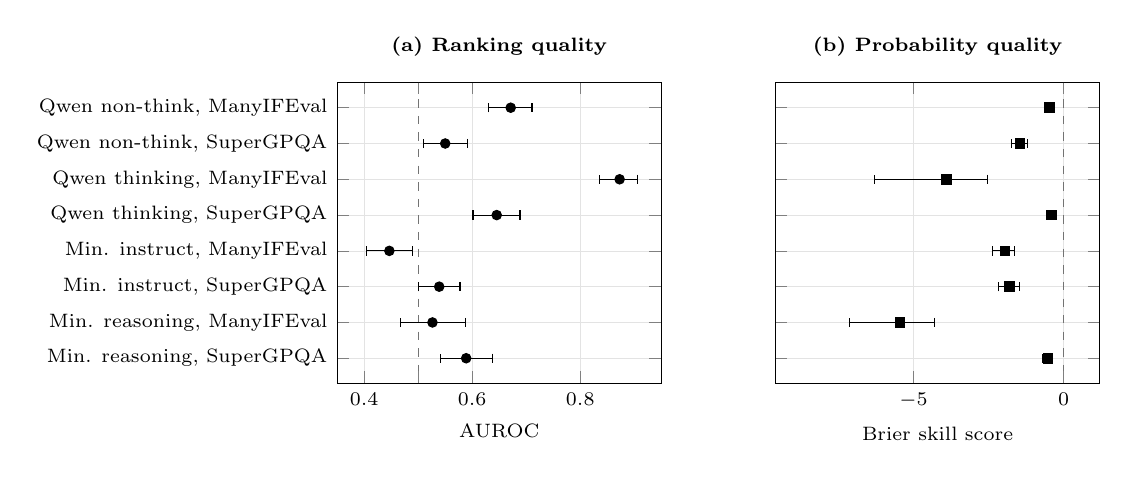
\begin{tikzpicture}
\pgfplotsset{
  cpisrow/.style={
    width=0.47\textwidth, height=5.4cm,
    ytick={0,1,2,3,4,5,6,7}, yticklabels={{Qwen non-think, ManyIFEval},{Qwen non-think, SuperGPQA},{Qwen thinking, ManyIFEval},{Qwen thinking, SuperGPQA},{Min. instruct, ManyIFEval},{Min. instruct, SuperGPQA},{Min. reasoning, ManyIFEval},{Min. reasoning, SuperGPQA}},
    y dir=reverse, ymin=-0.7, ymax=7.7,
    tick label style={font=\scriptsize}, label style={font=\scriptsize},
    title style={font=\scriptsize\bfseries},
    grid=major, grid style={gray!22,very thin},
  },
}
\begin{axis}[cpisrow, name=left, xlabel={AUROC}, title={(a) Ranking quality},
  xmin=0.35, xmax=0.95, extra x ticks={0.5}, extra x tick style={grid=major,
  grid style={black!55,dashed}, xticklabel=\empty}]
\addplot[only marks, mark=*, mark size=1.7pt, color=black,
  error bars/.cd, x dir=both, x explicit, error bar style={black}]
  coordinates {(0.6713,0) += (0.0395,0) -= (0.0409,0) (0.5501,1) += (0.0411,0) -= (0.0402,0) (0.8729,2) += (0.0325,0) -= (0.0376,0) (0.6454,3) += (0.0432,0) -= (0.0439,0) (0.4467,4) += (0.0427,0) -= (0.0426,0) (0.5390,5) += (0.0385,0) -= (0.0390,0) (0.5265,6) += (0.0610,0) -= (0.0594,0) (0.5889,7) += (0.0479,0) -= (0.0470,0)};
\end{axis}
\begin{axis}[cpisrow, at={(left.south east)}, xshift=1.45cm, anchor=south west,
  yticklabels=\empty, xlabel={Brier skill score}, title={(b) Probability quality},
  xmin=-9.6, xmax=1.2, extra x ticks={0}, extra x tick style={grid=major,
  grid style={black!55,dashed}, xticklabel=\empty}]
\addplot[only marks, mark=square*, mark size=1.7pt, color=black,
  error bars/.cd, x dir=both, x explicit, error bar style={black}]
  coordinates {(-0.4635,0) += (0.1127,0) -= (0.1272,0) (-1.4505,1) += (0.2322,0) -= (0.2756,0) (-3.8944,2) += (1.3576,0) -= (2.4000,0) (-0.4109,3) += (0.1117,0) -= (0.1174,0) (-1.9518,4) += (0.3235,0) -= (0.4105,0) (-1.7952,5) += (0.3135,0) -= (0.3803,0) (-5.4471,6) += (1.1453,0) -= (1.6982,0) (-0.5238,7) += (0.1478,0) -= (0.1699,0)};
\end{axis}
\end{tikzpicture}

\vspace{1.5ex}

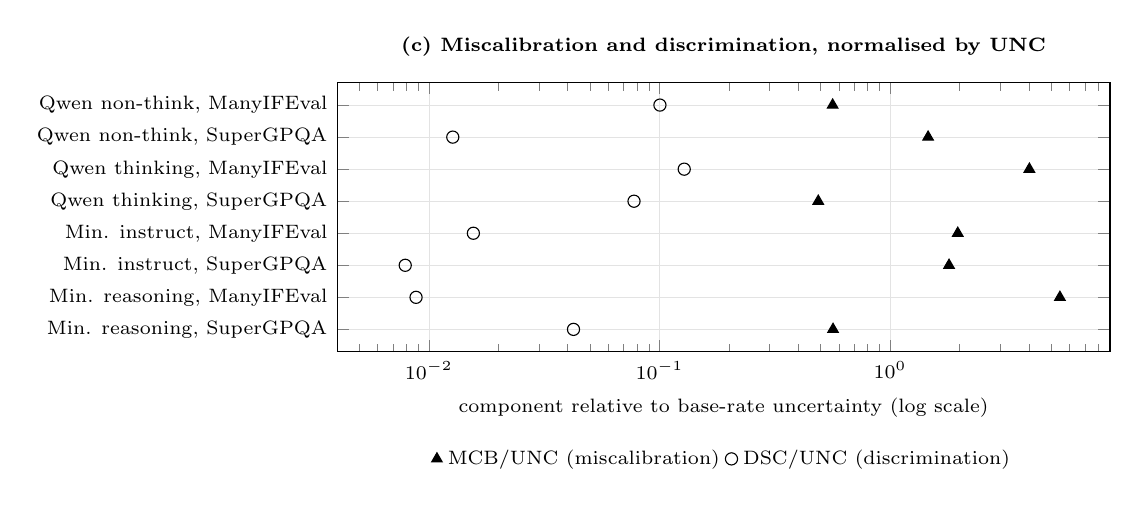
\begin{tikzpicture}
\begin{axis}[
  width=0.94\textwidth, height=5.0cm,
  ytick={0,1,2,3,4,5,6,7}, yticklabels={{Qwen non-think, ManyIFEval},{Qwen non-think, SuperGPQA},{Qwen thinking, ManyIFEval},{Qwen thinking, SuperGPQA},{Min. instruct, ManyIFEval},{Min. instruct, SuperGPQA},{Min. reasoning, ManyIFEval},{Min. reasoning, SuperGPQA}}, y dir=reverse,
  ymin=-0.7, ymax=7.7,
  xmode=log, xmin=0.004, xmax=9,
  xlabel={component relative to base-rate uncertainty (log scale)},
  title style={font=\scriptsize\bfseries},
  title={(c) Miscalibration and discrimination, normalised by UNC},
  tick label style={font=\scriptsize}, label style={font=\scriptsize},
  legend style={font=\scriptsize, at={(0.5,-0.32)}, anchor=north, legend columns=2, draw=none},
  grid=major, grid style={gray!22,very thin}]
\addplot[only marks, mark=triangle*, mark size=2.2pt, color=black] coordinates {(0.5640,0) (1.4631,1) (4.0225,2) (0.4885,3) (1.9675,4) (1.8031,5) (5.4559,6) (0.5662,7)};
\addlegendentry{MCB/UNC (miscalibration)}
\addplot[only marks, mark=o, mark size=2.2pt, color=black] coordinates {(0.1005,0) (0.0127,1) (0.1281,2) (0.0776,3) (0.0156,4) (0.0079,5) (0.0088,6) (0.0424,7)};
\addlegendentry{DSC/UNC (discrimination)}
\end{axis}
\end{tikzpicture}
